%!TEX root = ../ArticleCalib_main.tex

%%%%%%% CARACTERISATION OF SINGLE PIX RESPONSE article calib
\section{Single pixel response's characterisation \label{sec:SinglePixCaract}}

When considering the image obtained from a very dim object, the problem is to distinguish if a pixel or an area of pixels is significantly higher (or not) than the neighbours. In other words, is a pattern of pixels (zeros and ones) consistent with the random effect of a perfectly uniform optical field, or is it produced by a contrasted object ? 
To address an heterogeneous light flux detection, it is essential to know the background and the fluctuations of each pixel one by one. \par

We studied the camera pixels with the following steps. 
First, studying the global response of the detector (ones' frequency per frame for a given exposure time), gives a preliminary approach of the real CIC and $I_{d}$ of our camera (\ref{fig:PixByPix:A}).
Second, we determined for each pixel the CIC and the $I_{d}$ by a linear regression for exposure times that stay away from saturation ( \ref{fig:PixByPix:B}). For the linear regression, we weighted the estimated variance of each data point, and were satisfied with the goodness of fit ($\chi^2$, data not shown.) 
Then we observed the distribution of the  CIC and the $I_{d}$ parameters across all pixels (\ref{fig:PixByPix:B}), leading to a histogram (\ref{fig:PixByPix:F}, \ref{fig:PixByPix:G}) and cumulative distribution (\ref{fig:PixByPix:D}, \ref{fig:PixByPix:E})  and an image (data not shown) for each parameter. Abnormal pixels were localised on the camera chip, and subsequently discarded when needed.\par

The heterogeneity of the sensor shows outliers of lower $I_{d}$ (2\textperthousand, 513$^e$ line) and higher $I_{d}$, (1\textperthousand, randomly spread on the sensor), as well as pixels of higher CIC, patterned in pixels columns, with outliers among them ($\tilde{F}_{CIC} > 5.10^{-3}$ : 1\textperthousand, 513$^e$ line.) However, 99\% of the detector is homogeneous, with a noise variation coefficient $c_v$ such as $c_v_{CIC}$ = 0.32 and  $c_v_{Id}$ = 0.34. \par
\medskip

%%!TEX root = ../ArticleCalib_main.tex
%!TEX root = ../sections/articleCalib_section4_SinglePixResponse

%%%%%%% FIGURE 1  : SINGLE PIX RESPONSE / HISTO CDF

\newgeometry{top=10mm}

\begin{figure}[]
\begin{center}
\captionsetup[subfigure]{position=top, labelfont=bf, textfont=normalfont, singlelinecheck=off, justification=raggedright }

\subfloat[]{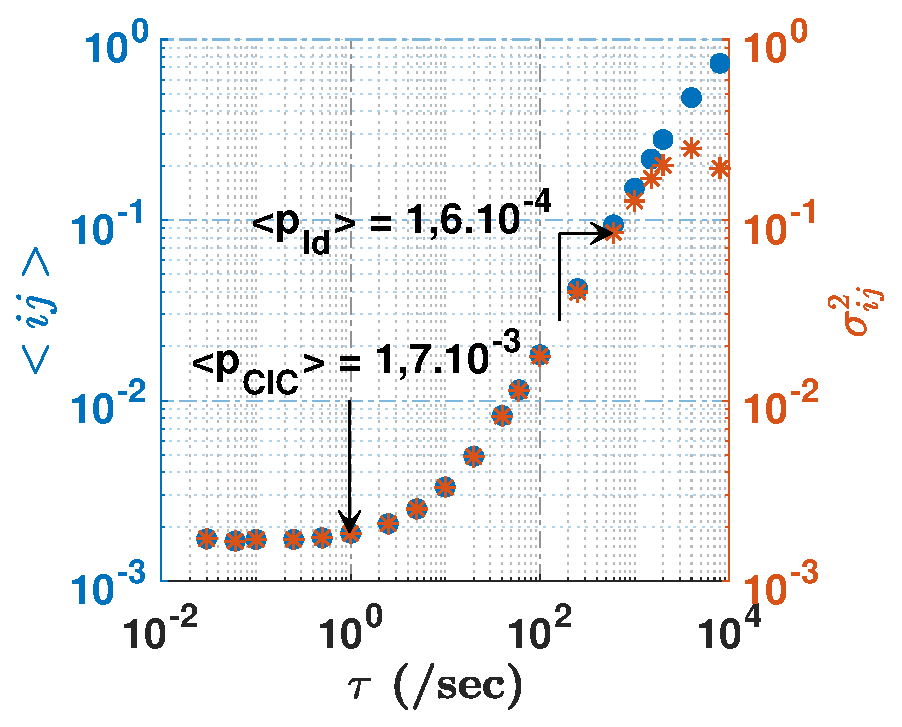
\includegraphics[width=0.40\linewidth]{fig1_caractSinglePixresponse/fig1A_meanvarIJ_Tau.eps}\label{fig:PixByPix:A}}  \\

\subfloat[]{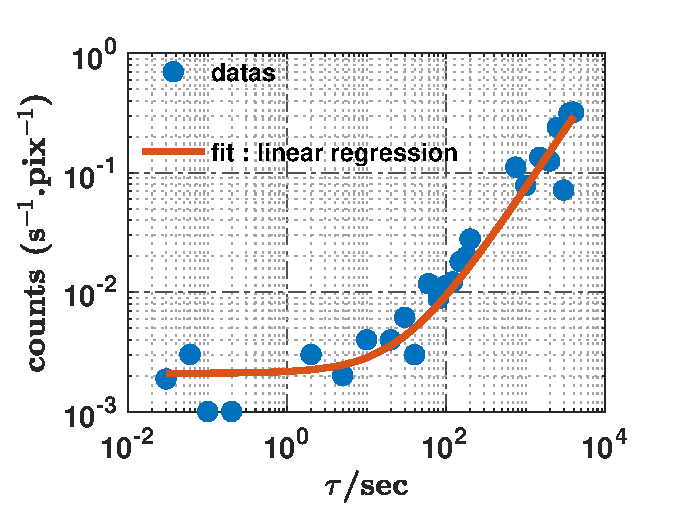
\includegraphics[width=0.40\linewidth]{fig1_caractSinglePixresponse/fig1B_fitmodel_MEF_170808_testLinFitWeighteddataPixIndex30010.eps}\label{fig:PixByPix:B}}\qquad
\subfloat[]{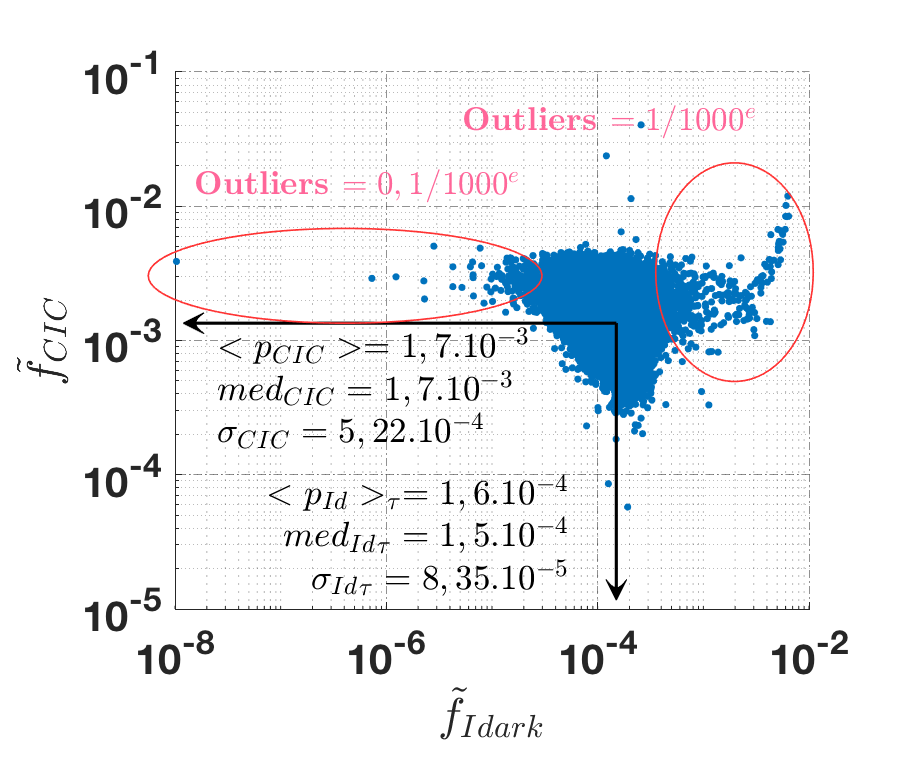
\includegraphics[width=0.4\linewidth]{fig1_caractSinglePixresponse/fig1C_PlotbiParam.eps}\label{fig:PixByPix:C}}  \\

\subfloat[]{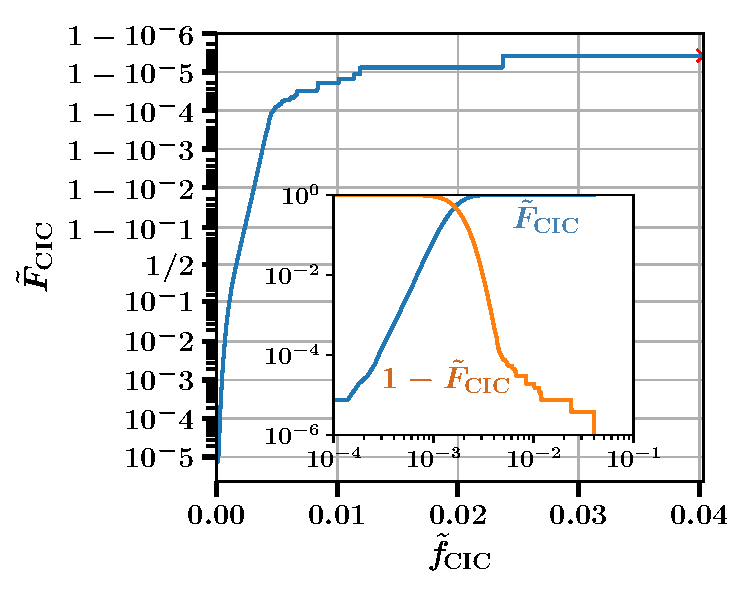
\includegraphics[width=0.40\linewidth]{fig1_caractSinglePixresponse/fig1D_E_CumSumCIC_Python.pdf}\label{fig:PixByPix:D}} \qquad
\subfloat[]{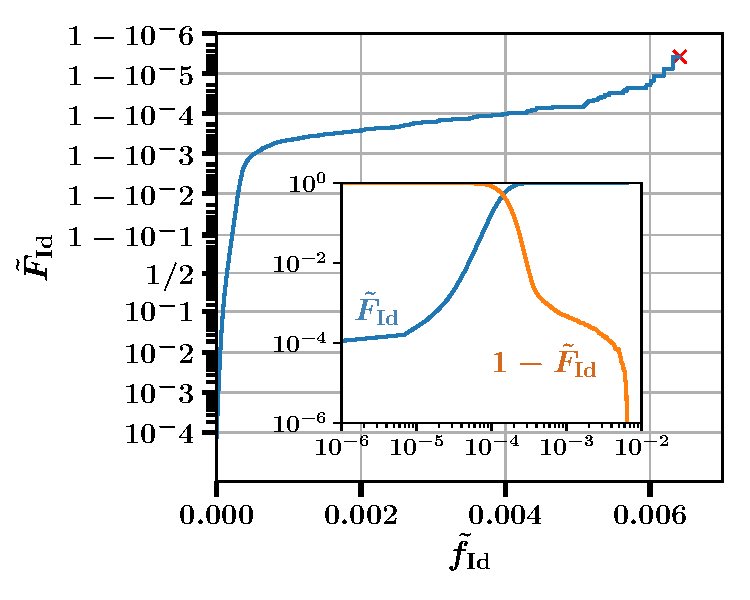
\includegraphics[width=0.40\linewidth]{fig1_caractSinglePixresponse/fig1D_E_CumSumId_Python.pdf}\label{fig:PixByPix:E}}. \\

\subfloat[]{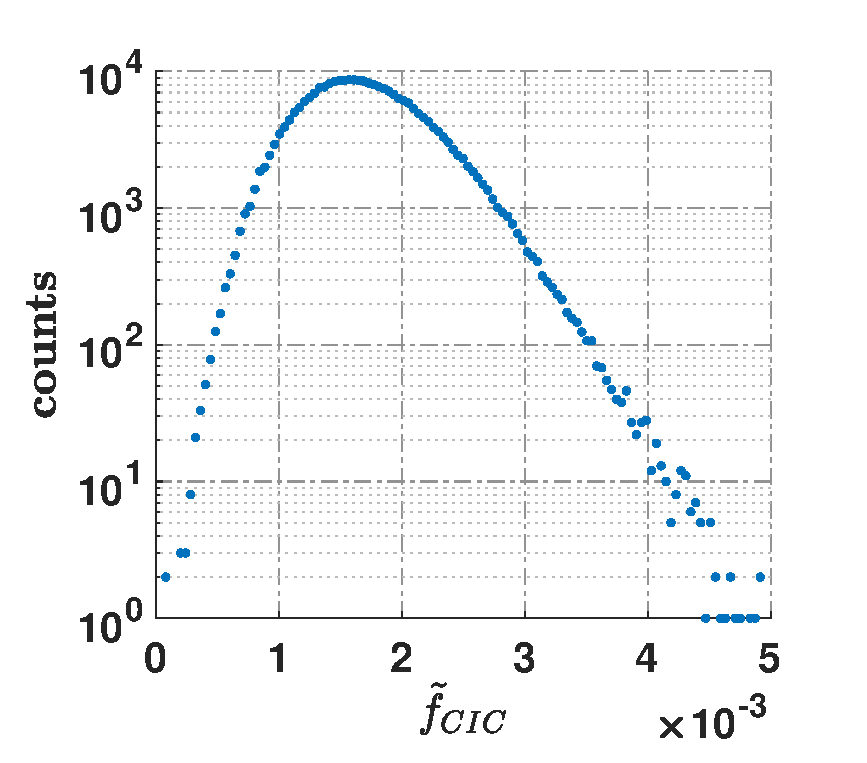
\includegraphics[width=0.35\linewidth]{fig1_caractSinglePixresponse/fig1F_G_HistoCIC.eps}\label{fig:PixByPix:F}} \qquad
\subfloat[]{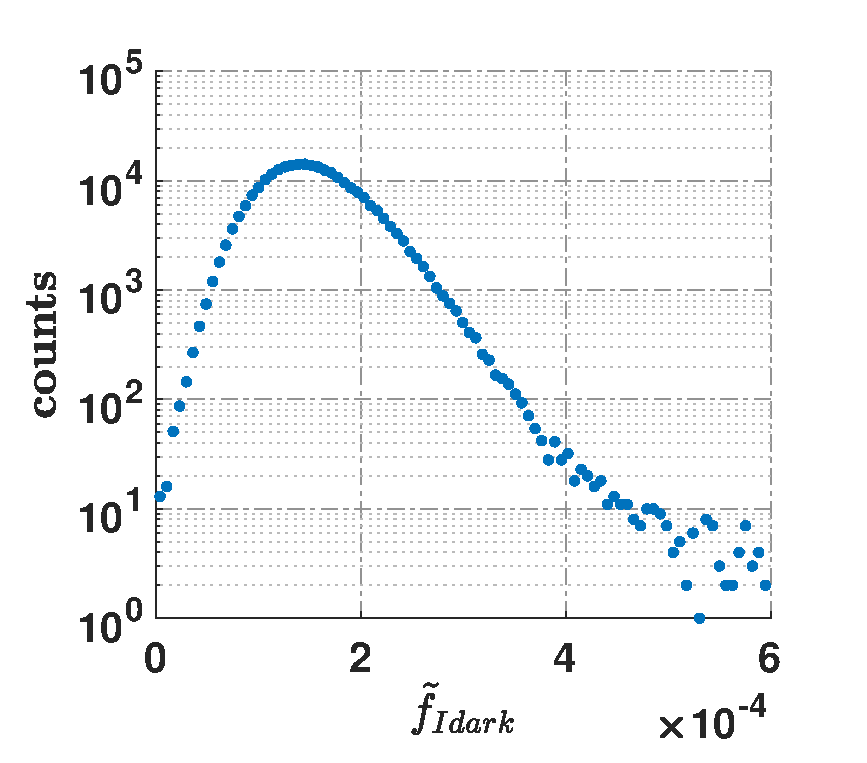
\includegraphics[width=0.35\linewidth]{fig1_caractSinglePixresponse/fig1F_G_HistoId.eps}\label{fig:PixByPix:G}} \\ 


\caption{{\bf Global detector response.} Evolution of the frequency of counts with the time of exposure  \subref{fig:PixByPix:A} .
{\bf single pixel : exemple of fit.} The individual pixel average noise response to an increased time of exposure $\tau$  was extracted and fitted out of saturation by weighted linear regression \subref{fig:PixByPix:B}. In those conditions the linear response is considered such as  <pixel$_{ij}$>$_K$$= CIC + Id * \tau$.
{\bf Caracterisation of single pixel response.} Single pixel response statistics \subref{fig:PixByPix:C}.  
Cumulative distribution (CDF) of the Clock Induced Charges (CIC) noise \subref{fig:PixByPix:D} and  the dark current (Id) \subref{fig:PixByPix:E} : Arctanh transform representation with insert in logarithmic scale  of the CDF and 1-CDF.
Histograms of the CIC \subref{fig:PixByPix:F} and the Id  \subref{fig:PixByPix:G}.}
\label{fig:PixByPix}
\end{center}
\end{figure}

\restoregeometry 



Analytically, a succession of ones and zeros has a frequency $p$ of ones and a variance $\sigma^2 = p(1-p)$ (figure \ref{fig:PoissonsIntervals:B} is a graphic representation of  $\sigma^2$ as a function of $p$ for all camera's pixels.) 
However, if this result is compatible with a pure Bernoulli, it doesn't inform about the history of pixels's counts.\par
To see if the noise of the detector is compatible with a poissonian distribution, we have to verify that the events are independents in time - history independent ; thus, we looked at the distribution of time intervalles between two pixel's count, for all pixels, and for different exposure times.(\ref{fig:PoissonsIntervals:A}.) 
As the CIC and $I_{d}$ parameters are projected on the Bernoulli parameter of the pixel for one given exposure time,  we can't extract them analytically from the fit. Also, we can't explain the factor 2 found for the fit parameter during short exposure time.  This distribution doesn't show temporal irregularities from minority pixels, fits well with an exponential function, and is therefore compatible with a truncatedPoisson distribution as described in the model. \par

Those parameters were finally integrated in our SNR model to simulate the response of our specific camera and, when used at its best, its capacity limits to detect low light fluxes.


%%!TEX root = ../ArticleCalib_main.tex
%!TEX root = ../sections/articleCalib_section4_SinglePixResponse


%%%%%%%%%%%%% FIGURE 2 BERNOUILLI POISSON INTERVALLES


\begin{figure}[htbp]
\begin{center}
\captionsetup[subfigure]{position=top, labelfont=bf, textfont=normalfont, singlelinecheck=off, justification=raggedright }

\subfloat[]{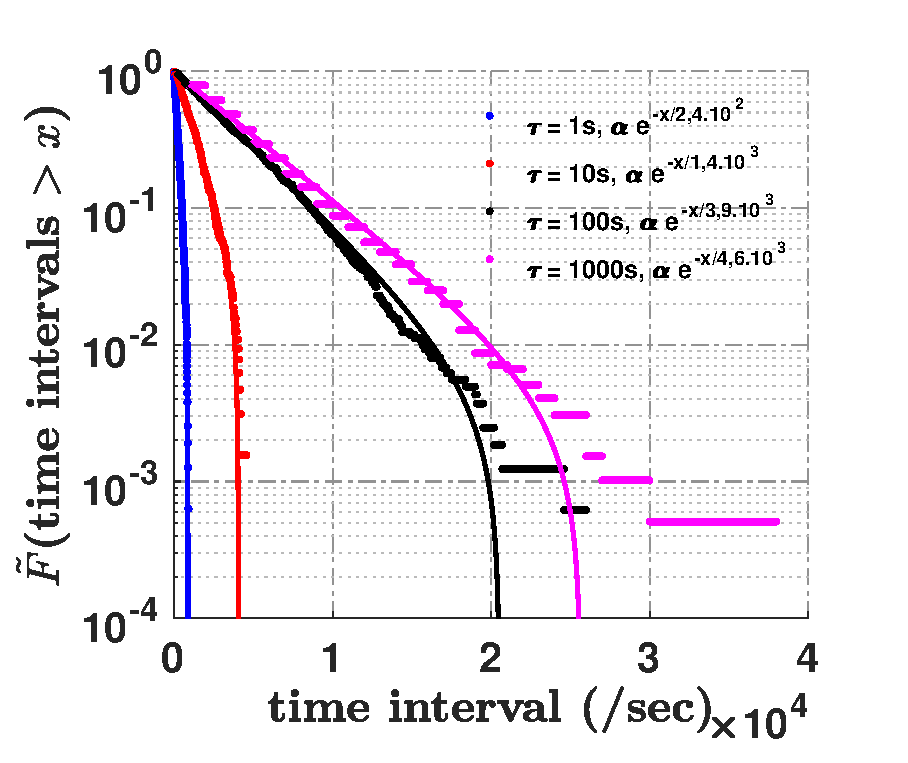
\includegraphics[width=0.4\linewidth]{fig2_ArgumentCompatiblesPoiss/fig2_Poiss_distriIntervalles.eps}\label{fig:PoissonsIntervals:A}}  
%\qquad
%\subfloat[]{\includegraphics[width=0.4\linewidth]{fig2_ArgumentCompatiblesPoiss/anlz_varmeanij_yxline_varexcess.eps}\label{fig:PoissonsIntervals:B}}  \\


\caption{{\bf Distribution of time intervals.} The complement of the cumulative distribution of the time intervals between two successive counts for a pixel$_{ij}$ for all pixels is represented. The time intervals are exctracted for differents times of exposure $\tau$ and fitted by an exponential model. For each $\tau$, the time constant found according to the model is given \subref{fig:PoissonsIntervals:A}} 
%{\bf All pixels are perfect Bernouilli.} The pixels can only take values 1 and 0. By definition they can be only fellow a  bernouilli law with  $\sigma_{ij_K}^2 = <$pixels$_{ij}>_K * (1-<$pixels$_{ij}>_K) $ strictly \subref{fig:PoissonsIntervals:B}. }

\label{fig:PoissonsIntervals}
\end{center}
\end{figure}
%%%%%%%%%%%%%%%%%%%

 	



